\documentclass[11pt]{article}
\renewcommand{\baselinestretch}{1}
\usepackage[utf8]{inputenc}
\usepackage[parfill]{parskip}
\usepackage{graphicx}
\usepackage{amsmath}
\usepackage{caption}
\captionsetup[table]{position=bottom} 
\usepackage[title]{appendix}
\usepackage[margin=25mm]{geometry}
\usepackage{amsmath,graphicx,psfrag,pstricks}
\def\n{\noindent}
\def\u{\underline}
\usepackage{gensymb}
\def\hs{\hspace}
\newcommand{\thrfor}{.^{\displaystyle .} .}
\newcommand{\bvec}[1]{{\bf #1}}
\usepackage{graphicx}
\usepackage{rotating}
\graphicspath{{Plots/}}
\usepackage{amsmath}
\usepackage{booktabs}
\usepackage{siunitx}
\usepackage{amssymb}
\usepackage[utf8]{inputenc}
\usepackage[justification=centering]{caption}
\usepackage{float}
\usepackage{listings}
\usepackage{color} %red, green, blue, yellow, cyan, magenta, black, white
\definecolor{mygreen}{RGB}{28,172,0} % color values Red, Green, Blue
\definecolor{mylilas}{RGB}{170,55,241}
\lstset{language=Matlab,%
    %basicstyle=\color{red},
    breaklines=true,%
    morekeywords={matlab2tikz},
    keywordstyle=\color{blue},%
    morekeywords=[2]{1}, keywordstyle=[2]{\color{black}},
    identifierstyle=\color{black},%
    stringstyle=\color{mylilas},
    commentstyle=\color{mygreen},%
    showstringspaces=false,%without this there will be a symbol in the places where there is a space
    numbers=left,%
    numberstyle={\tiny \color{black}},% size of the numbers
    numbersep=9pt, % this defines how far the numbers are from the text
    emph=[1]{for,end,break},emphstyle=[1]\color{red}, %some words to emphasise
    %emph=[2]{word1,word2}, emphstyle=[2]{style},  
}
\title{Part IIA Project - GF1: Control Systems - Second Interim Report}
\author{Bailey Brookes | Corpus Christi | bdb31}
\date{\today}

\begin{document}

\maketitle

\section{Controlling the separator level}

\subsection{Proportional Control}

\subsubsection{Heuristic Method}
By adding a slider gain to provide negative feedback and a step input to provide the L2 set-point, such as that show in the handout, trial and error can be used to get the response of the F2-L2 loop to have a 50\% overshoot. The gain that achieves this is -48 and is shown in Figure \ref{L2_man}.

The effect of a $\pm10\%$ change in set point is shown in Figure \ref{L2_setpoints}.These response are the same response but mirrored about the 1m nominal set-point, and both give under/overshoot of 50\% as required.

The effect of a $\pm10\%$ change in the flow rate F1 is shown in Figure \ref{F2_setpoints}. Interestingly, even though the separator acts like an integrator, there is still steady state error when F1 is change. This is discussed later in the report and fixed with a proportional integral (PI) control.

\subsubsection{Theoretical Method}
The bode plot for the linearised version of the F2-L2 loop is shown in Figure \ref{OG_bode}. For a phase margin at $45\degree$, the gain plot needs to be raised by 22.9dB which is equivalent to a gain of -13.9. The response of the L2-F2 loop with this gain is shown in Figure \ref{L2_theory} and the bode plot in Figure \ref{-13.9_bode}. 

There is a large difference between the heuristic and theoretical gain, with the theoretical gain giving less overshoot but the required set point and phase margin. The heuristic gain of -48 gives a phase margin of 28\degree, 62\% of what it should be. 

\subsection{Proportional and Integral Control}
Changing the F1 flow rate as shown in Figure \ref{F2_setpoints} changes the L2 set-point. Despite an integrator in the separator, there is still steady state error. This is because the integral control removes steady state error by ensuring the sum between set point and curve reaches zero so acts on the error output signal to change the error signal. So feedback is required. The integrator in the separator isn't used in feedback so doesn't remove the steady state error. 

To remove the steady state error an integrator in the control loop is required. The specifications require a phase margin of 40\degree with the integral action in the control, which is the same as having a phase lag of 5\degree at the frequency which gives a phase margin of 45\degree, which is 0.595 rad/s. To calculate T$_i$ in the handout, we solve:

\begin{gather*}
1 - j\frac{1}{0.595T_i} = \tan5\degrees \hspace{1cm} \implies \hspace{1cm} T_i = 19.2
\end{gather*}

The response of this PI controller is shown in Figure \ref{PI_set}, demonstrating that the controller removes the steady state error caused by varying the flow rate F1. The bode plot, which shows that the phase margin is around 40\degree, is shown in Figure \ref{PI_bode}.

\section{Constraints on Variables}
Adding constraints on variable makes the model more realistic as many inputs will have maximum or minimum values, be it by design or available input. For example, the feed flow rate can only increase by so much and cannot be negative so is limited to 0 to 20 kg/min.

\subsection{Changing X1}
The L2-F2 controller is very robust to step changes in X2. The nominal value is 5\% and the controller behaves well up to 23\% and down to 0\%, which is shown in Figure \ref{X2_Levels}.

\subsection{Changing F1}
The L2-F2 controller is much less robust in changes to F1, failing to control the set-point above 12kg/min and below 8kg/min, shown in Figure \ref{F2_Levels}.

\appendix

\section{Plots}
\begin{figure} [H]
\centering	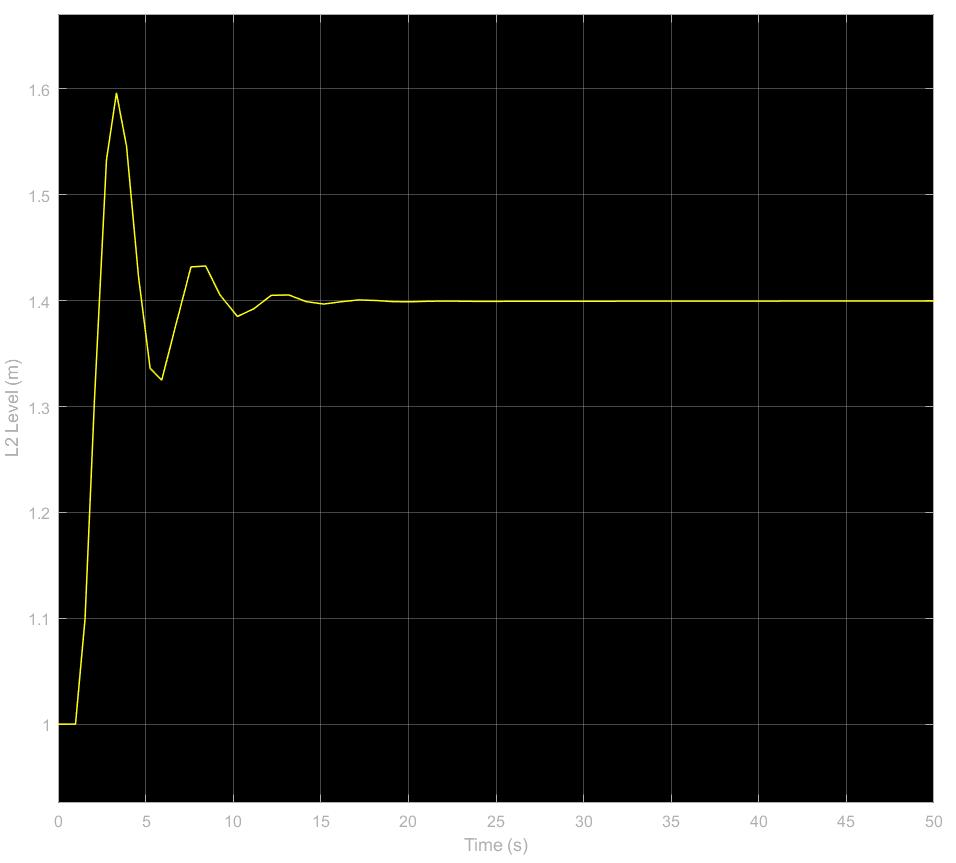
\includegraphics[scale = 0.3]
{L2_control_maual}
\caption{Response of the L2-F2 control loop with gain of -48}
\label{L2_man}
\end{figure}

\begin{figure} [H]
\centering	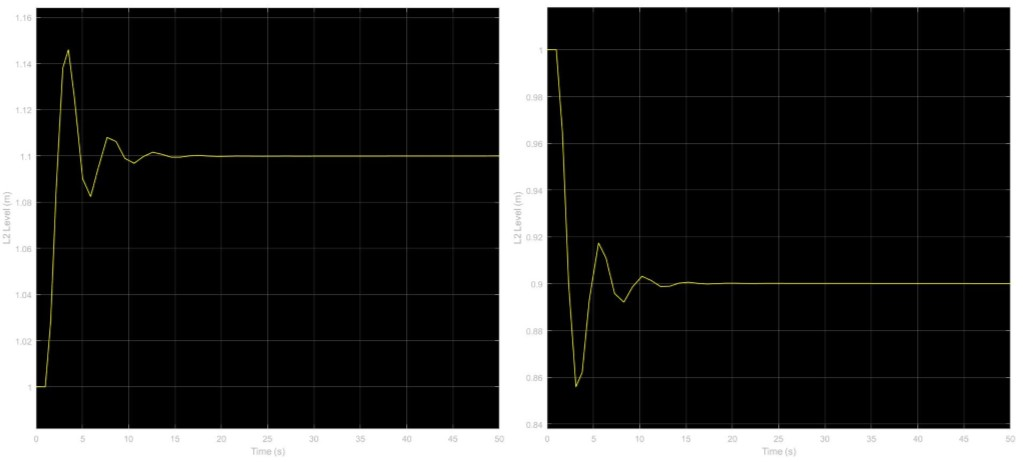
\includegraphics[scale = 0.6]
{L2_setpoints}
\caption{Response of the heuristic designed L2-F2 control loop at set-pint of L2 to 1m (left) and 0.9m (Right)}
\label{L2_setpoints}
\end{figure}

\begin{figure} [H]
\centering	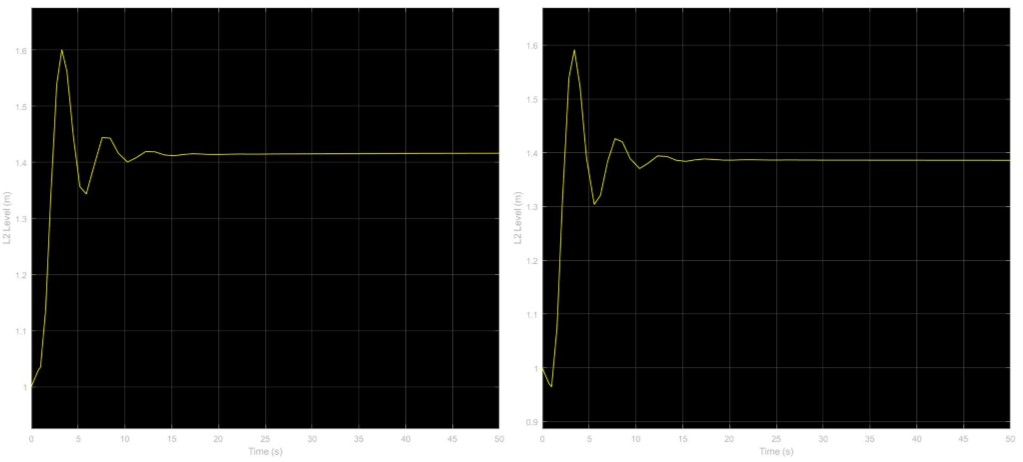
\includegraphics[scale = 0.6]
{F2_setpoints}
\caption{Response of the heuristic designed L2-F2 control loop at set-pint of F2 to 11kg/min (left) and 9kg/min (Right)}
\label{F2_setpoints}
\end{figure}

\begin{figure} [H]
\centering	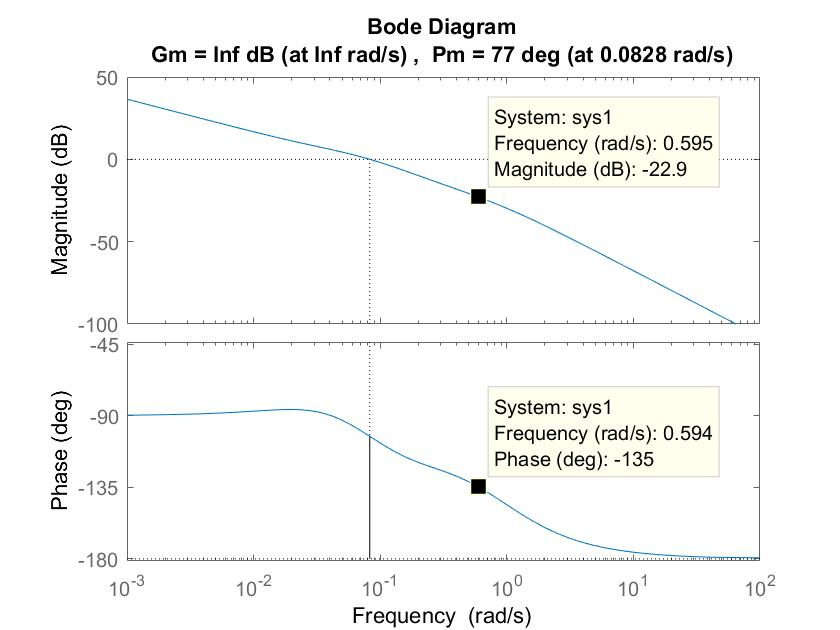
\includegraphics[scale = 0.4]
{L2_Open_bode}
\caption{Bode plot of the open F2-L2 loop}
\label{OG_bode}
\end{figure}

\begin{figure} [H]
\centering	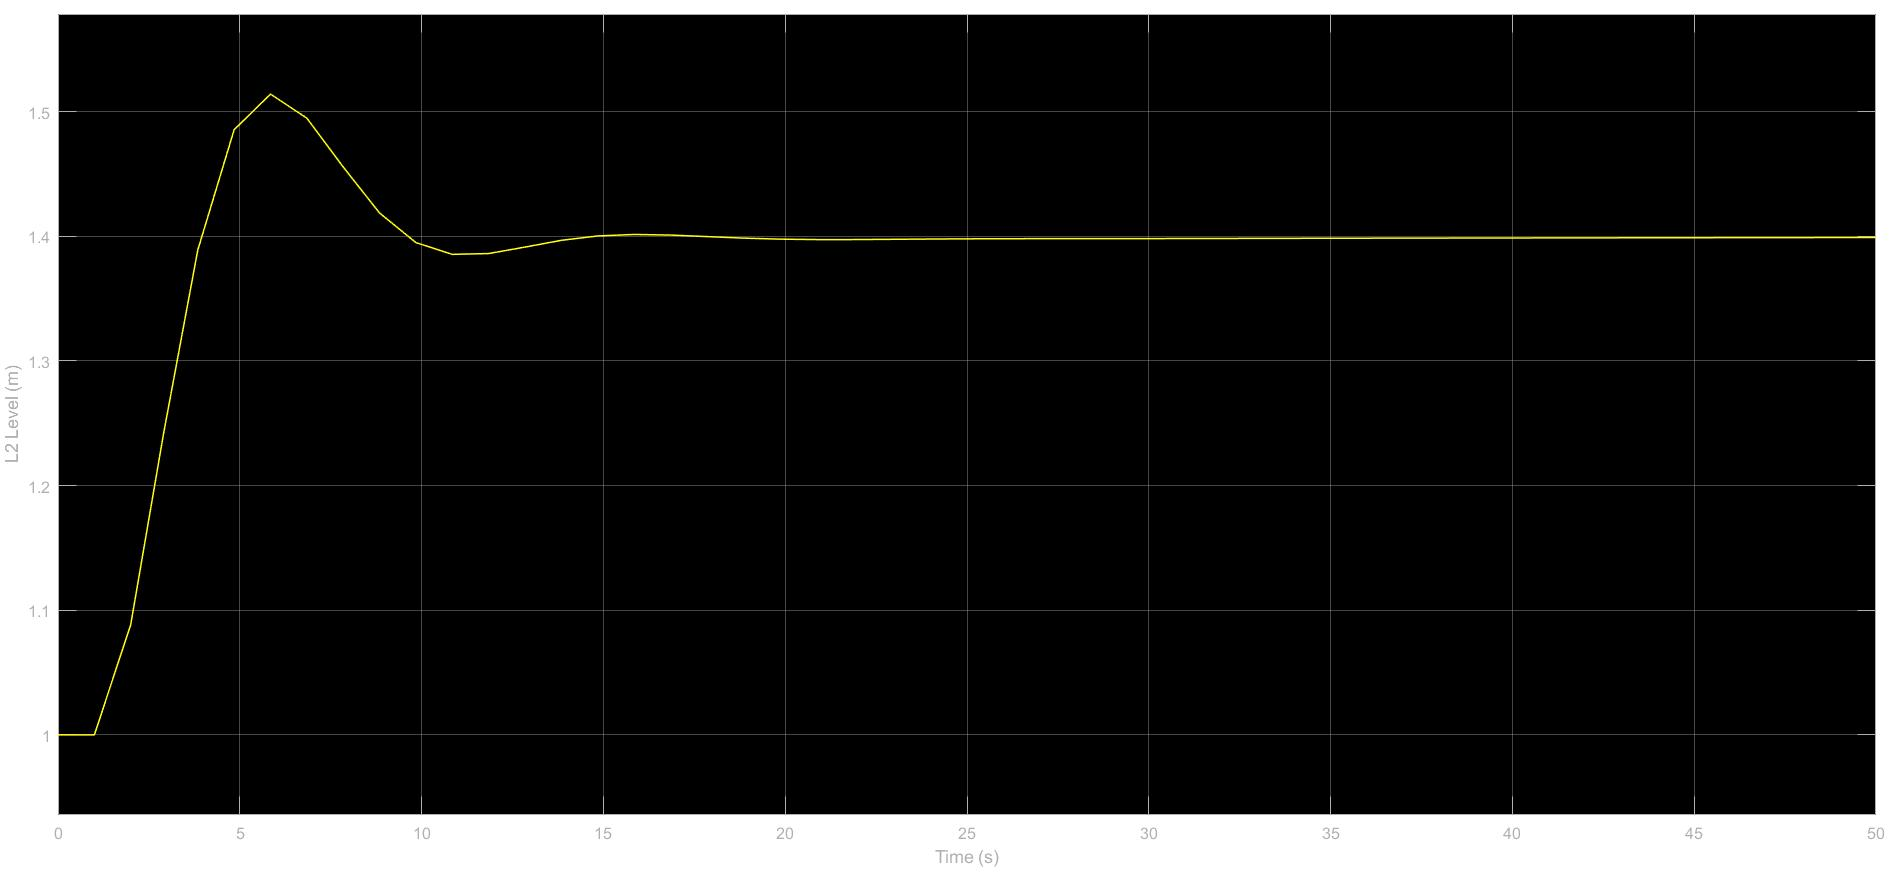
\includegraphics[scale = 0.2]
{L2_theory}
\caption{Response of the L2-F2 control loop with gain of -13.9}
\label{L2_theory}
\end{figure}

\begin{figure} [H]
\centering	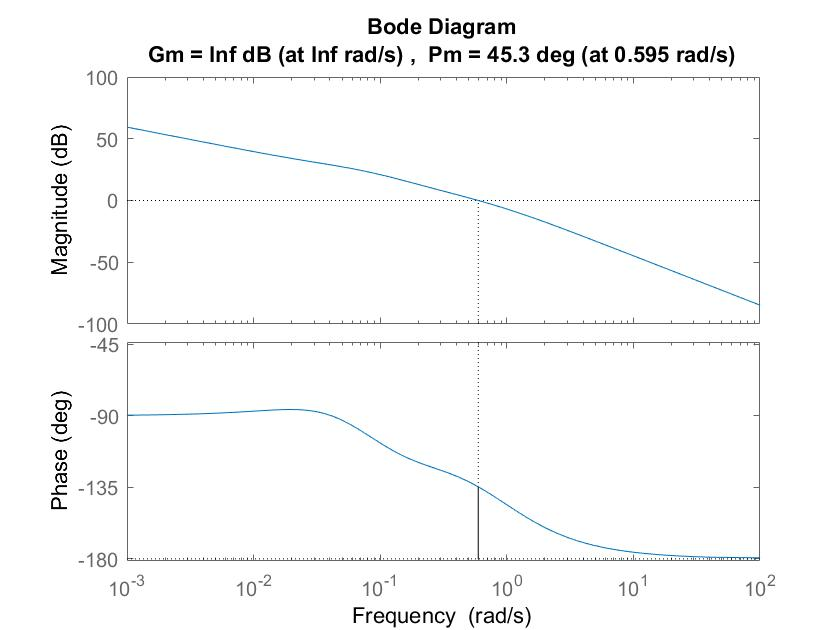
\includegraphics[scale = 0.4]
{L2_139_bode}
\caption{Bode plot of the open F2-L2 loop with gain of -13.9}
\label{-13.9_bode}
\end{figure}

\begin{figure} [H]
\centering	\includegraphics[scale = 0.6]
{PI_set}
\caption{Response of the L2-F2 control loop with PI control}
\label{PI_set}
\end{figure}

\begin{figure} [H]
\centering	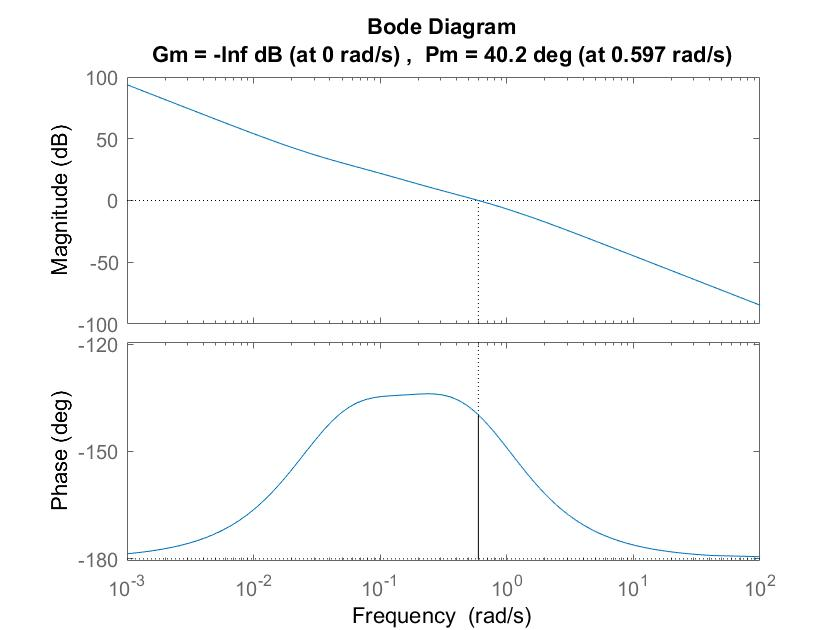
\includegraphics[scale = 0.4]
{L2_PI_Bode}
\caption{Bode plot of the open F2-L2 loop with PI control}
\label{PI_bode}
\end{figure}

\begin{figure} [H]
\centering	\includegraphics[scale = 0.6]
{PI_set}
\caption{Response of the L2-F2 control loop with PI control}
\label{PI_set}
\end{figure}

\begin{figure} [H]
\centering	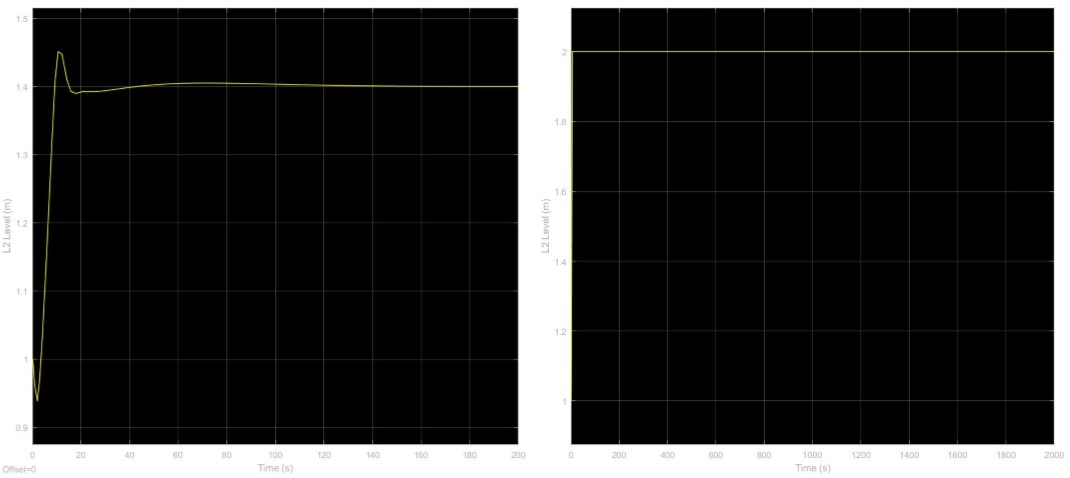
\includegraphics[scale = 0.6]
{X2_levels}
\caption{Response of the L2-F2 control loop with PI control for X1 at 0\% (Left) and 40\% (Right)}
\label{X2_Levels}
\end{figure}

\begin{figure} [H]
\centering	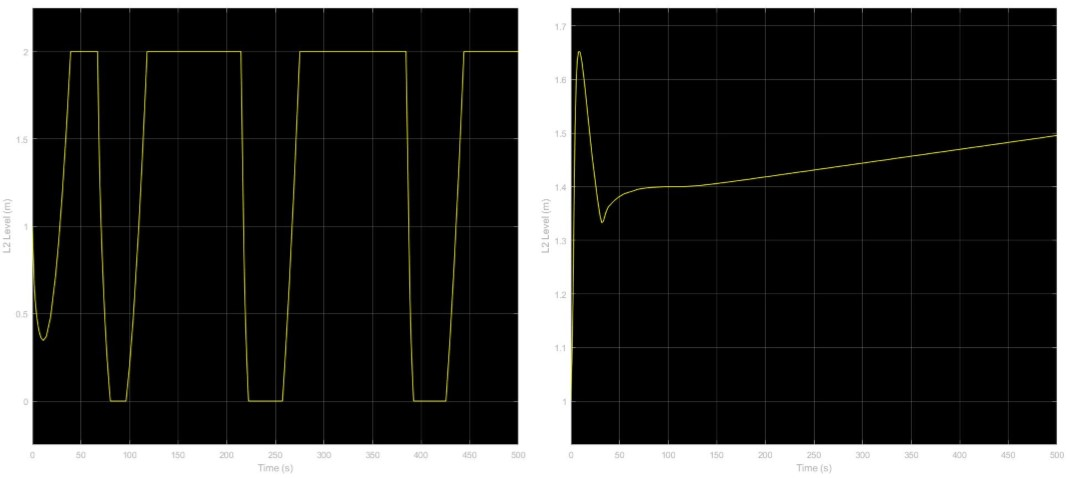
\includegraphics[scale = 0.6]
{F2_levels}
\caption{Response of the L2-F2 control loop with PI control for F1 at 7kg/min (Left) and 12.32kg/min (Right)}
\label{F2_Levels}
\end{figure}

\section{Simulink Models}
\begin{figure} [H]
\centering	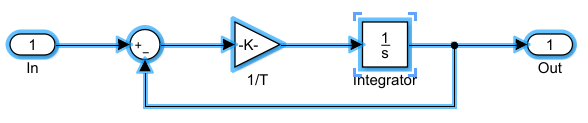
\includegraphics[scale = 0.5]
{servo}
\caption{Model of the delay caused by the servos}
\label{F2_Levels}
\end{figure}

\begin{figure} [H]
\centering	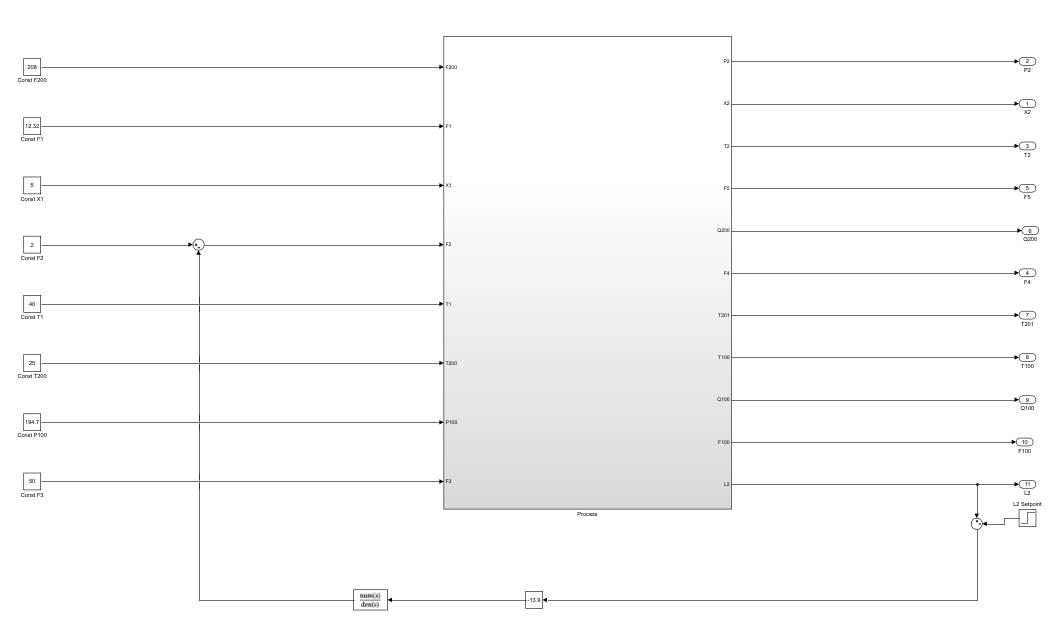
\includegraphics[scale = 0.7]
{process}
\caption{Model of the process at nominal values with servos and L2-F2 control}
\label{F2_Levels}
\end{figure}
\end{document}
